\documentclass[footheight=20pt, footsepline, headheight=20pt, headsepline]{scrartcl}
%
\usepackage[utf8]{inputenc} % below are various important packages
\usepackage{lmodern}
\usepackage[T1]{fontenc}
\usepackage[english]{babel}
\usepackage{textcomp} 
\usepackage{amsmath}
\usepackage{mathrsfs}
\usepackage{latexsym}
\usepackage{amssymb}	
\usepackage{amsfonts}
\usepackage{theorem}
\usepackage{graphicx}
\usepackage{scrlayer-scrpage}
\usepackage{xcolor}
\usepackage{setspace}
\usepackage{framed}
\usepackage{hyperref} 
\usepackage{pgf,tikz,pgfplots} % possibility to insert geogebra graphs
\usepackage{mathrsfs}
\pgfplotsset{compat=1.15}\usetikzlibrary{arrows} % part of geogebra package
\usepackage{qrcode} % insert qr codes
\usepackage{multicol}
\usepackage{multirow}
\usepackage{xurl}
\usepackage{tabularx}
\usepackage{enumitem}
\usepackage{float}

% Add to length for wider margins
\addtolength{\textwidth}{3cm} % right to margin
\addtolength{\hoffset}{-1.6cm} % left to margin
\addtolength{\voffset}{-2cm} % to top
\addtolength{\textheight}{6.5cm} % to bottom

% Headers-Footers
\definecolor{gro}{gray}{0.6} % define color
\setkomafont{pagehead}{\normalfont\sffamily} % define header
\setkomafont{pagefoot}{\normalfont\sffamily} % define footer
\addtokomafont{headsepline}{\color{gro}} % define header horizontal line
\addtokomafont{footsepline}{\color{gro}} % define footer horizontal line
	\ihead{\color{gro} AE-468 Final Report} % header (i=inner=left)
	\ohead{\color{gro} Cool Aircraft Name} % header (o=outer=right)
	\ifoot{\color{gro} } % footer (i=inner=left)
	\cfoot{\color{gro} - {\textbf\thepage} -} % footer (c=center)
	\ofoot{\color{gro} } % footer (o=outer=right)


\renewcommand{\familydefault}{\sfdefault} % font
\linespread{1.2} % increase line spacing

%---------------------------------------------------------------------------
\begin{document} % every document starts with \begin{document}
%\doublespacing
\title{
Cool Aircraft Name \\[1cm]
 \large{\textbf{Final Project Report} \\[1cm] Caroline Franklin, Kyle Torries, Wei Min Patrick}\\
 
 \begin{figure}[h]
 \centering
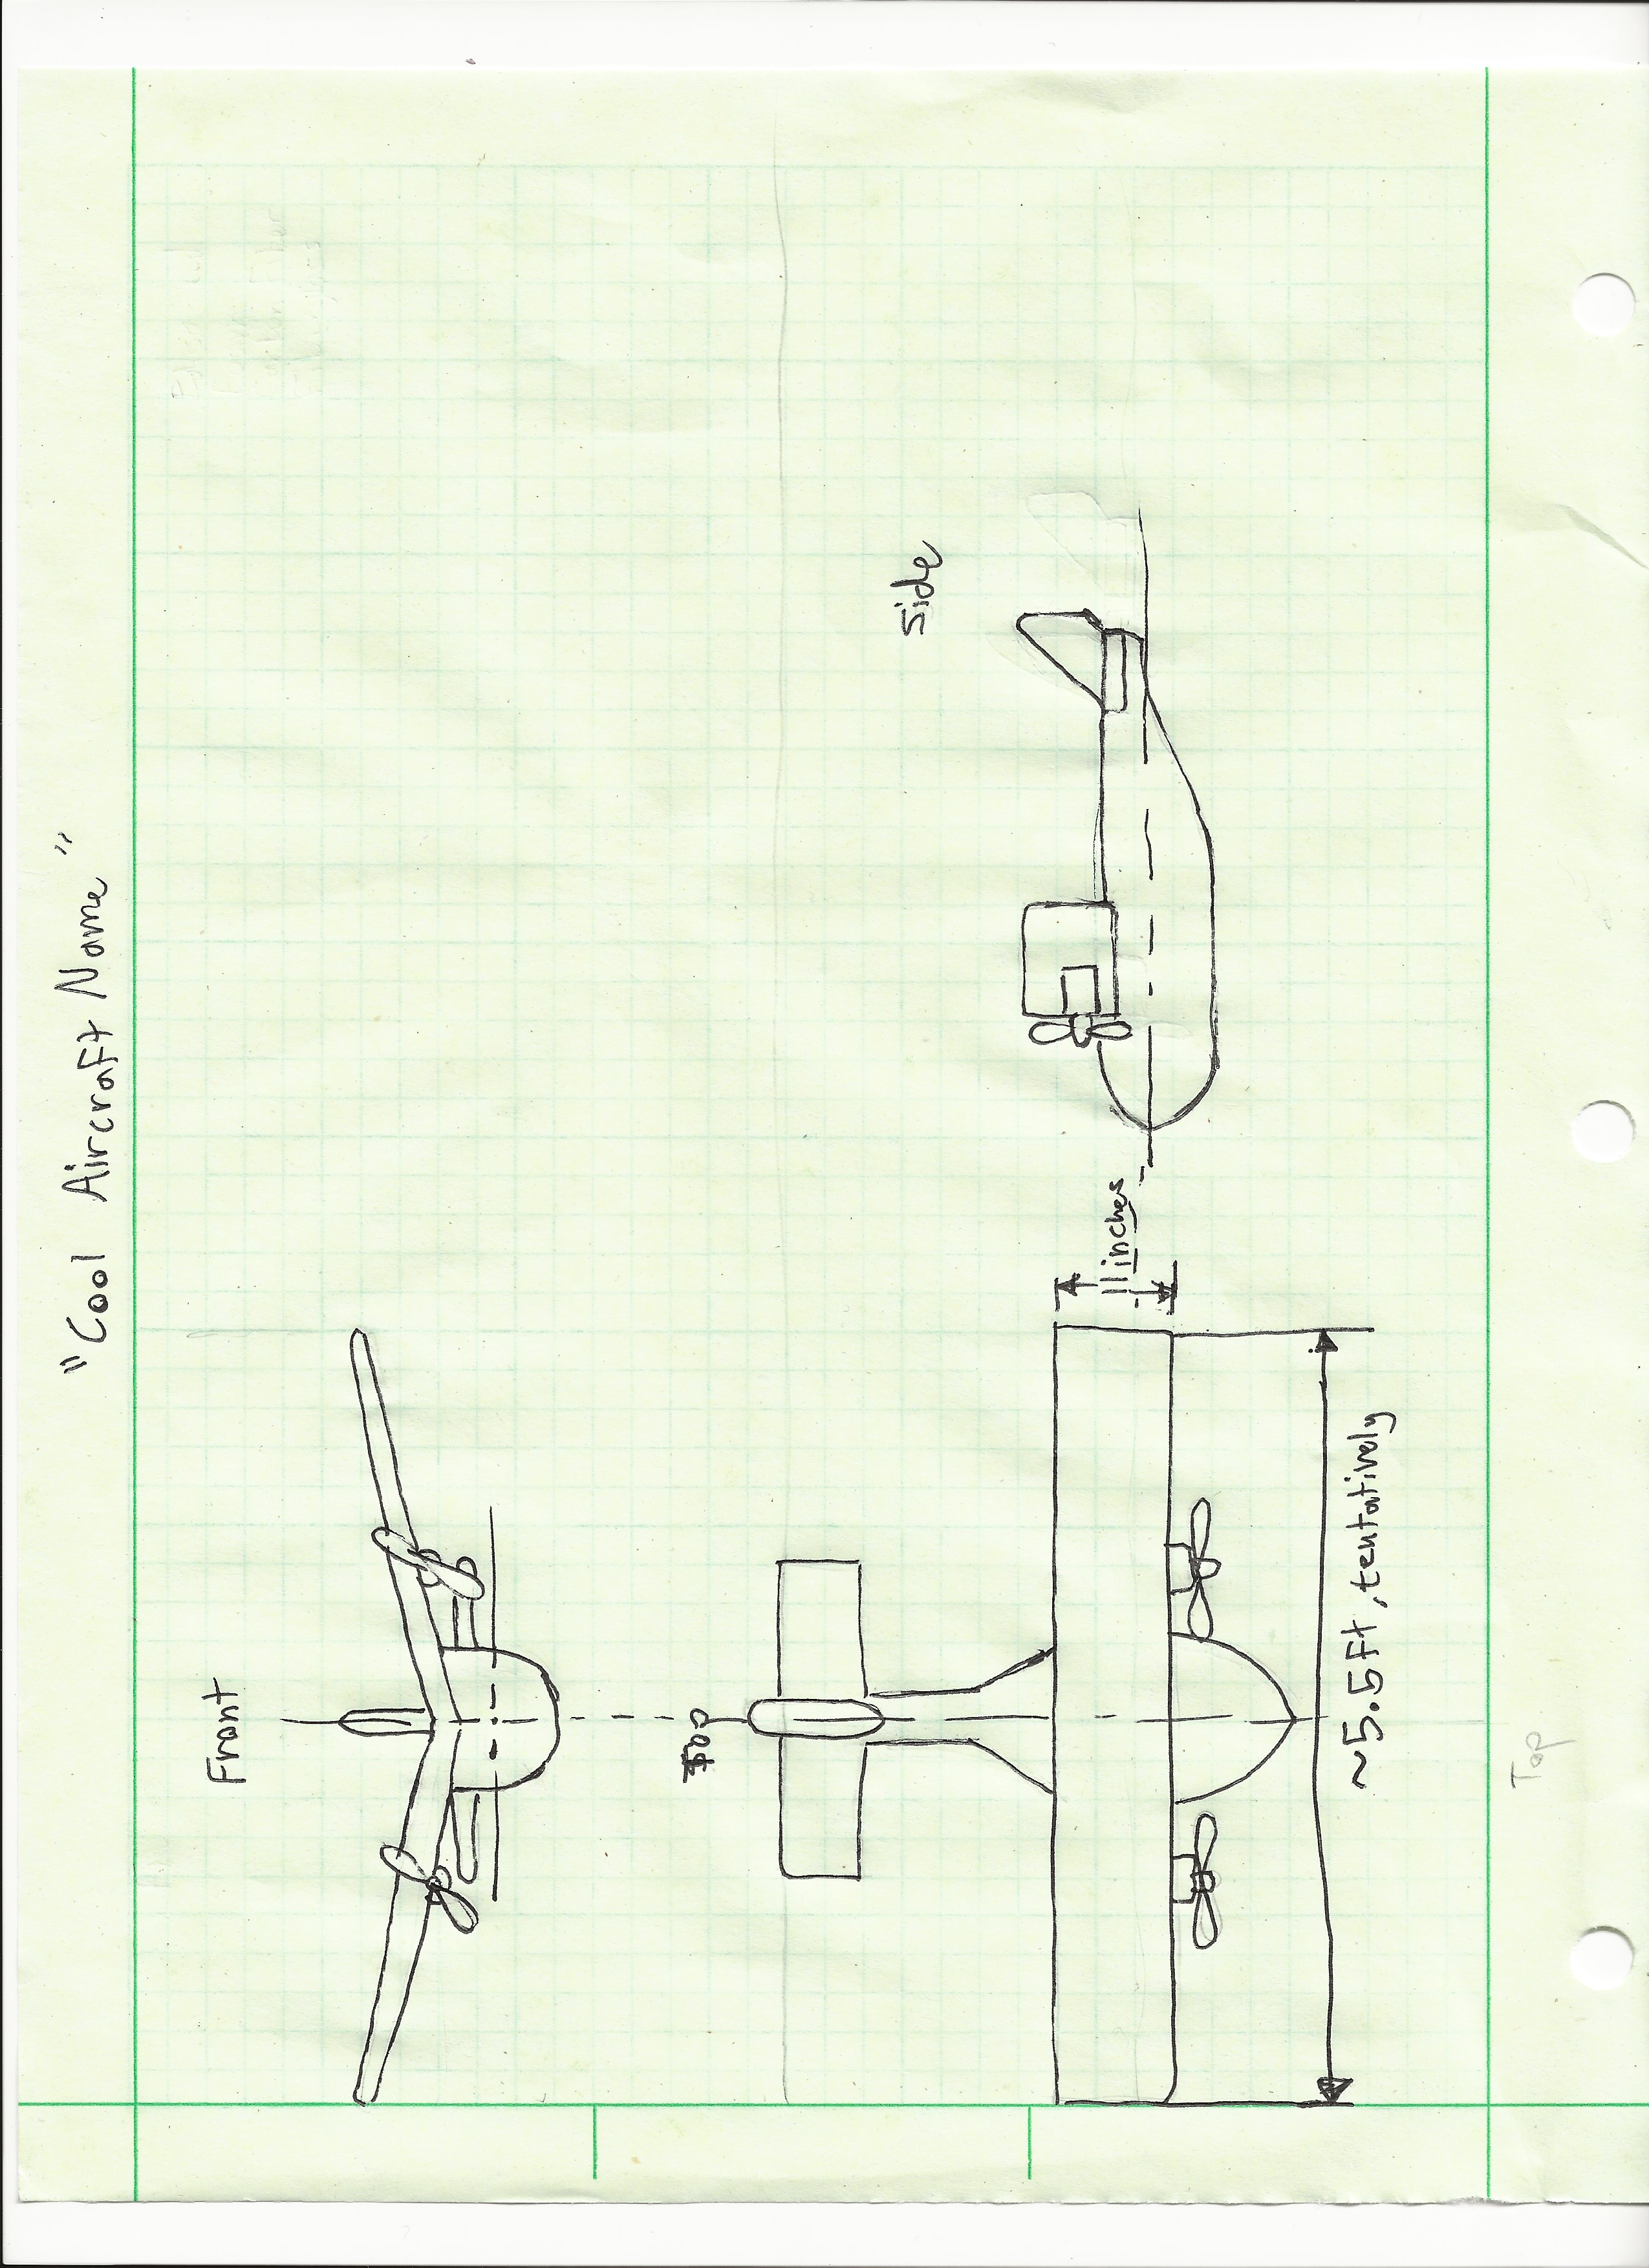
\includegraphics[width=9cm, height=13cm, angle=270]{cool aircraft name.jpeg}
\end{figure}} 

\date{\vfill \\University of South Alabama \\[0.5cm] AE-468 Aircraft Design \\[0.5cm] Spring Semester 2022}
\maketitle
%---------------------------------------------------------------------------
\newpage
\tableofcontents
%---------------------------------------------------------------------------
\newpage
\section{Executive Summary}
{The initial concept for the \textit{Cool Aircraft Name} is to have a glider-like design with a large wingspan to increase its surface area. The main goal is to design something that will more than likely be able to take off and land no matter the circumstances. This includes conditions such as weather, shelf life, or even minor damage to the aircraft before flight. It was suggested by the team that an aspect ratio of around 6 should be used to ensure stability, yet remain relatively easy to turn. The team has opted to use a dihedral, rectangular main wing located at the top of the fuselage. The plan is also to implement two propellers, each located on opposite sides of the main wing. The aircraft will also implement one horizontal stabilizer, one vertical stabilizer, and one tail boom. The team has chosen carbon fiber as the main material for the vehicle, however, this is subject to change depending on pricing. This material was chosen for its durability and weight. Additionally, it was discussed that data may be taken during the flight by implementing a Circuit Playground Bluefruit and IMU as the payload. This is also up for discussion as the team continues the designing process. The team discussed technology availability and believes all materials discussed are available because of the design's simplicity.} 
%---------------------------------------------------------------------------
\section{Aspect Ratio}
The formula for the aspect ratio is a follows:\begin{center}
\begin{equation}
AR = b^2/S
\end{equation}
\end{center}
where AR is the aspect ratio, b is the wing span, and S is the horizontal surface area of the wing and any other dedicated contact surfaces. The team decided that the goal for the aspect ratio is to be around 6, thus, by using an estimated wing span of around 5.5 ft, the area of the wing was calculated as follows:

\begin{equation}
\begin{array}{lcl}
S = b^2/AR \\
S = (5.5 ft)^2 /6 \\
S = 5.04 ft^2
\end{array}
\end{equation}

Thus, the height or chord, c, of the wing is,
\begin{equation}
\begin{array}{lcl}
c = S/b \\
c = 5.04 ft^2/5.5 ft \\
c = 0.916 ft
\end{array}
\end{equation}
%---------------------------------------------------------------------------
\section{Block Definition Diagram}
\centering
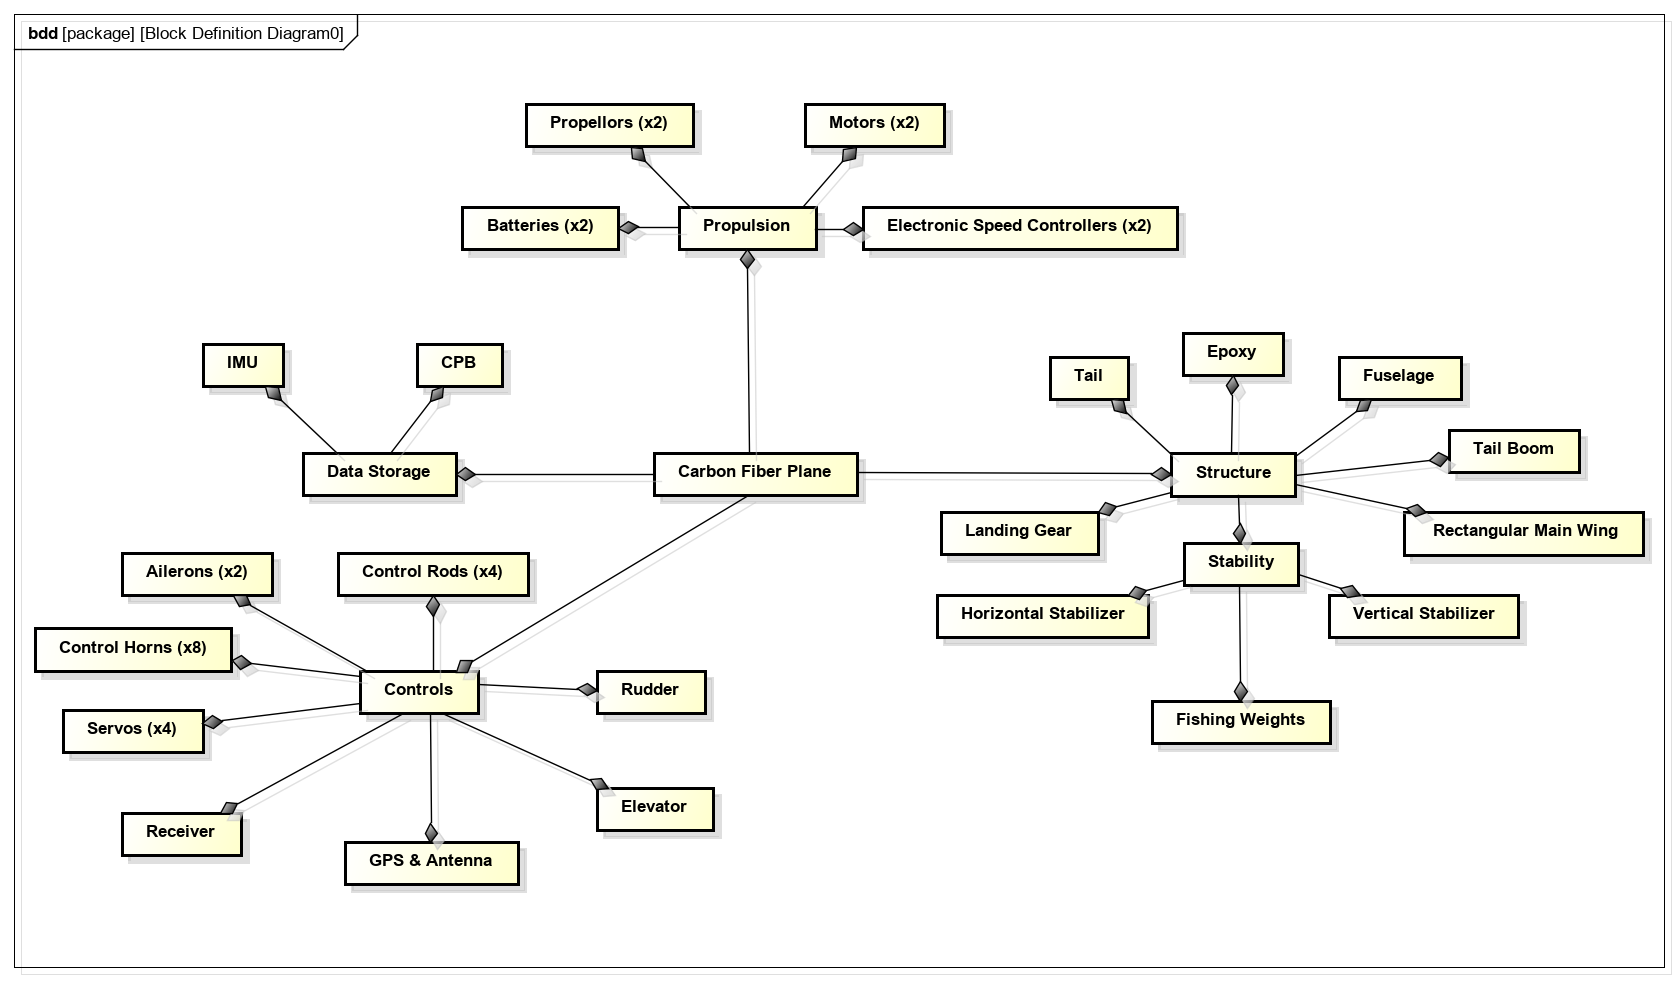
\includegraphics[width=18cm, height=15cm]{image (2).png}
%---------------------------------------------------------------------------
\section{3D-View Image by Kyle}
\centering
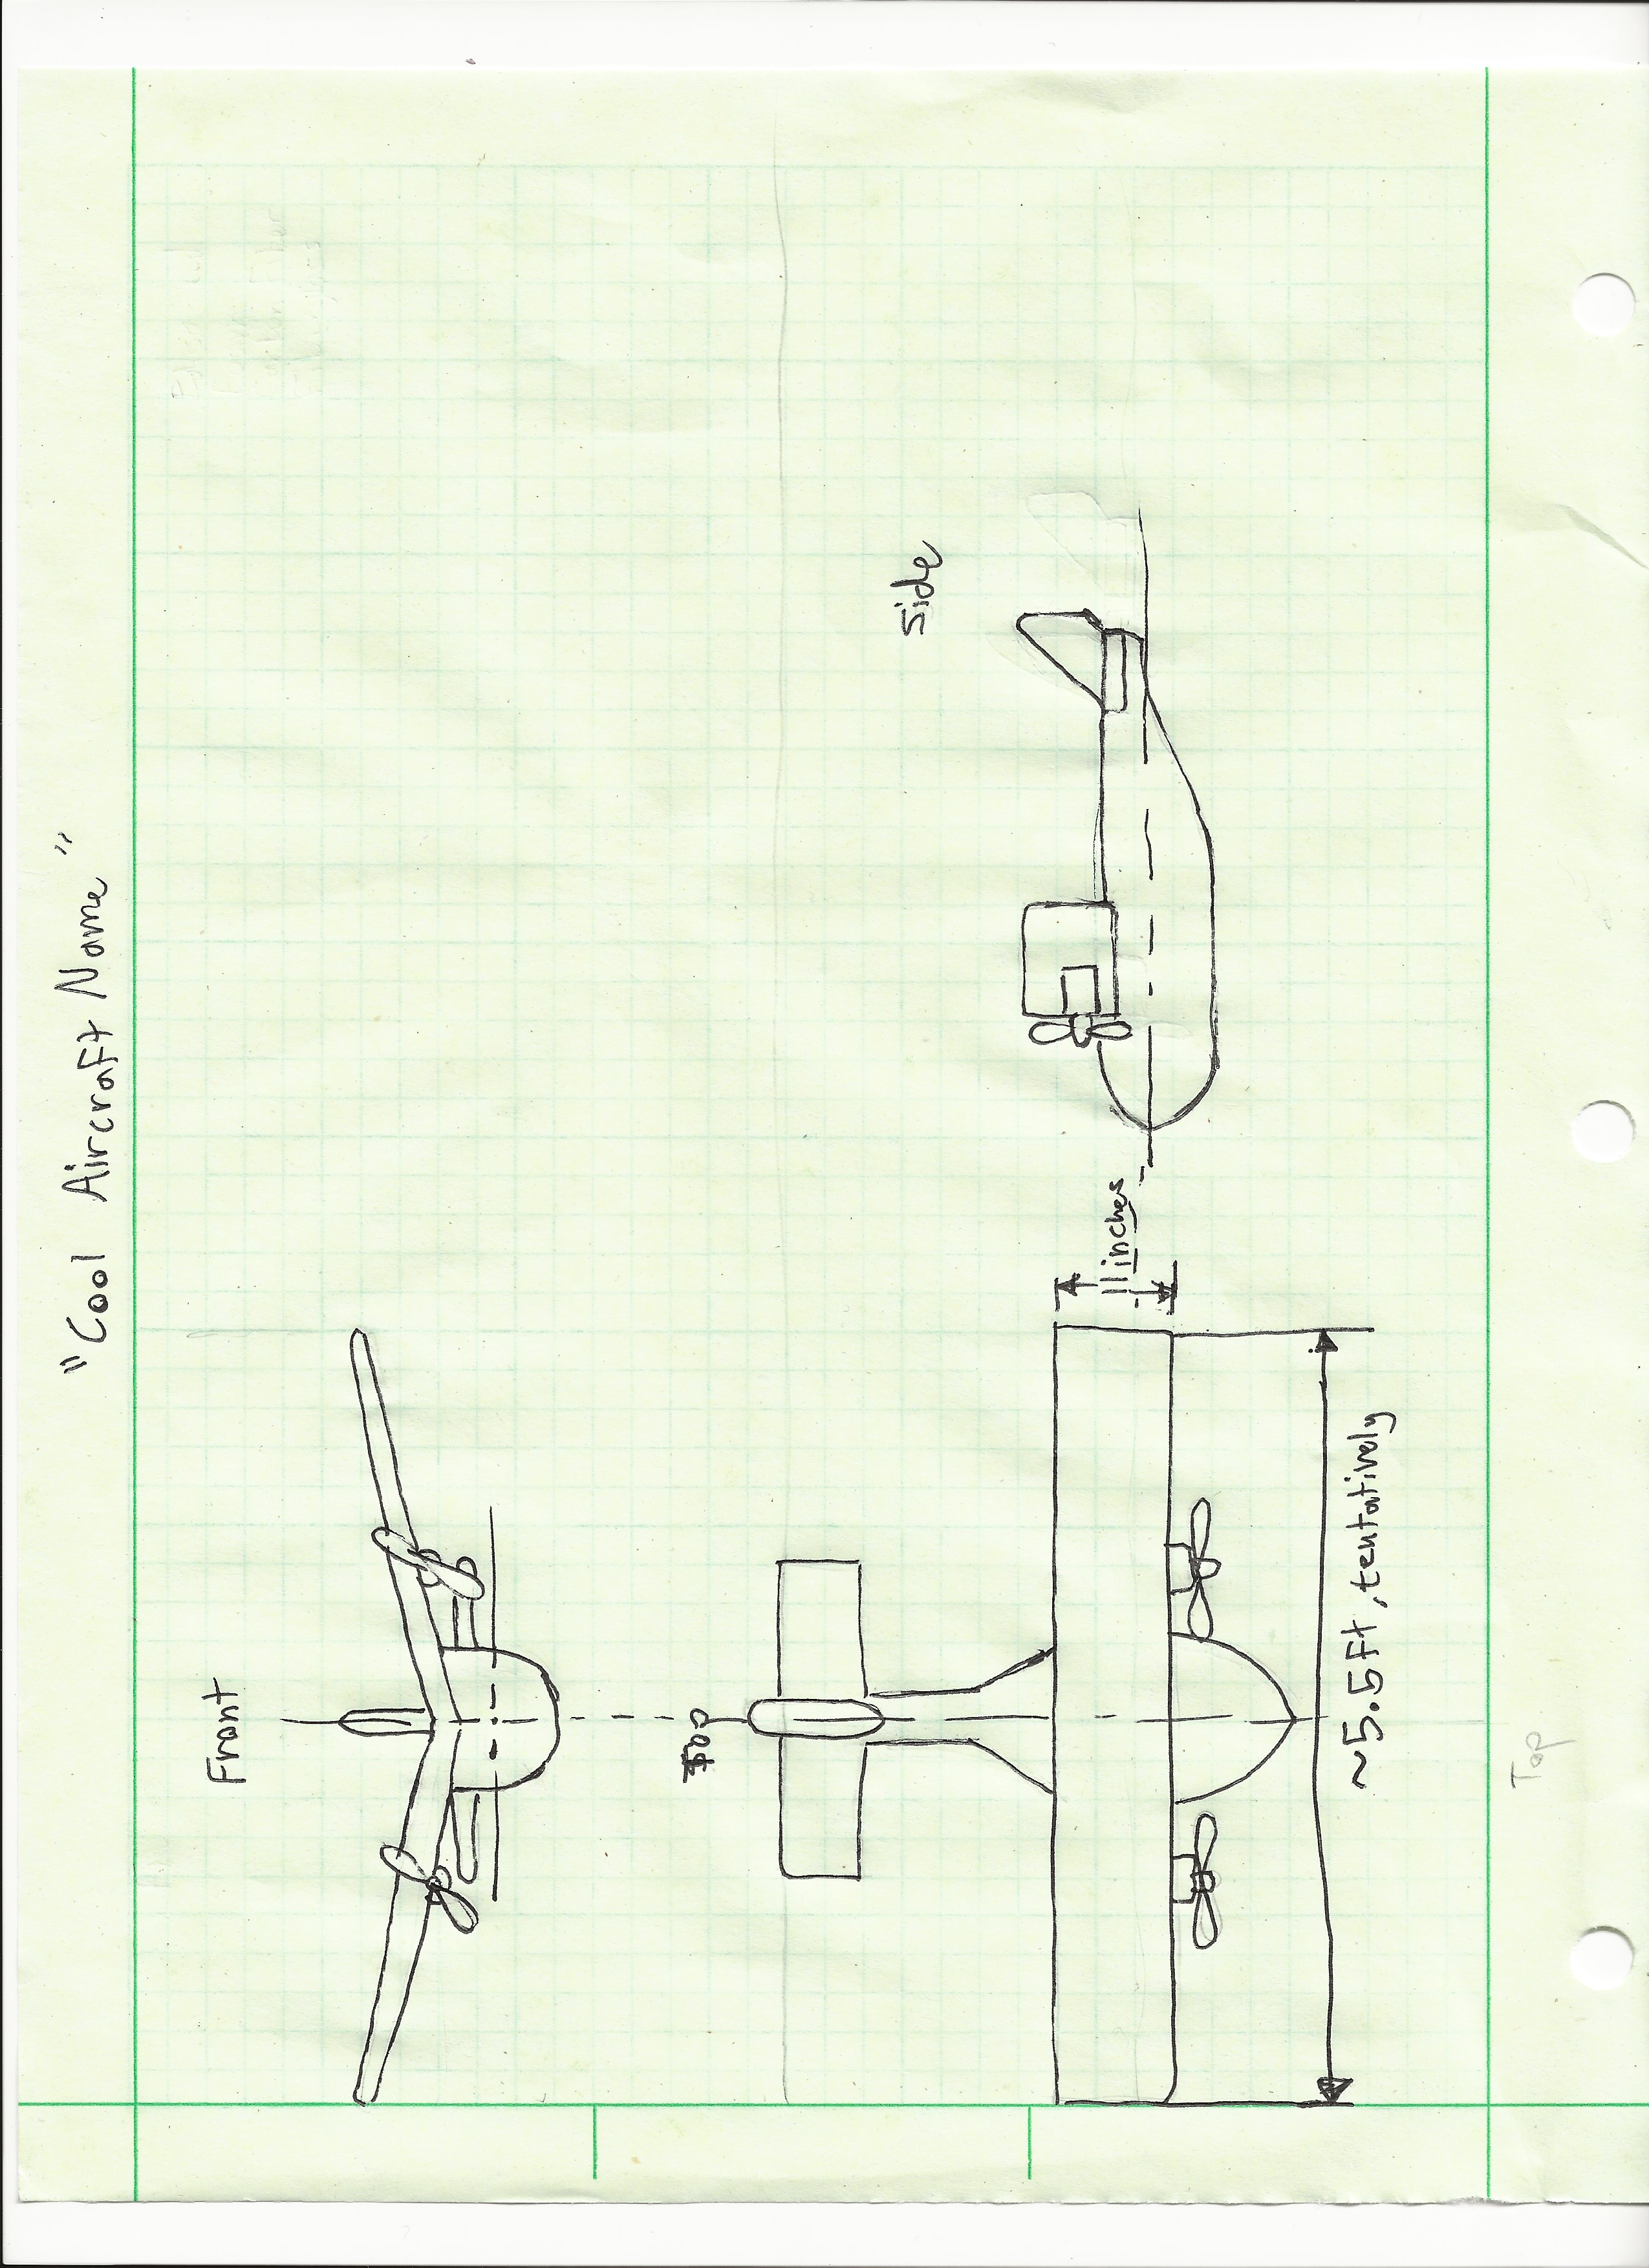
\includegraphics[width=10cm, height=15cm, angle=270]{cool aircraft name.jpeg}
%---------------------------------------------------------------------------
\newpage
\section{Component List}
\begin{table}[h!]
\begin{center}
\caption{Component list for Cool Aircraft Name}
\label{tab:table1}
\begin{tabular}{l|c|r} % <-- Alignments: 1st column left, 2nd middle and 3rd right, with vertical lines in between
% \\ is for making new rows, & is for making new columns
Component & Quantity \\
Propeller & 2 \\
Motor & 2 \\
Electronic Speed Controller & 2 \\
Tail Boom & 1 \\
Fuselage & 1 \\
Receiver & 1 \\
Radio & 1 \\
Elevator & 1 \\
Ailerons & 2 \\
Rudder & 1 \\
Control Rods & 4 \\
Control Horns & 8 \\
Servos & 4 \\
Battery & 2 \\
Main Wing & 1 \\
Vertical Stabilizer & 1 \\
Horizontal Stabilizer & 1 \\
CPB & 1 \\
IMU & 1 \\
Data Storage & 1 \\
GPS + Antenna & 1 \\
Carbon Fiber & 1 roll \\
Epoxy & Varies \\
Fishing Weights & Varies \\
Tape & 1 roll \\
Landing Gear & 1\\
\end{tabular}
\end{center}
\end{table}

\end{document}
